\chapter{序論}
\label{chap:introduction}
\minitoc

\thispagestyle{empty}

\newpage
%%%%%%%%%%%%%%%%%%%%%%%%%%%%%%%%%%%%%%%%%%%%%%%%%%%%%%%%%%%%%%%%%%%%%%%%%%%%%%%%%%%%%%%%%%%%%%%%%%%%%%%%%%%%%%%%%%%%%%%%%%%%%%%%%%%
\section{背景}
\label{sec:background_chap1}
現在,日本国内において脳血管疾患の患者数は約118万人存在する\cite{厚労省2014}.
脳血管疾患の一つである脳卒中は一旦発症すると,意識障害,運動障害,感覚障害など様々な障害を呈し,後遺症により麻痺が残る場合がある.
麻痺により寝たきり状態や介護が必要となるとなると日常生活に支障をきたしてしまう.
脳卒中は介護が必要になった原因の第二位であり,第一位の認知症の18.0 \%に次いで全体の16.6 \%を占める\cite{厚労省2016}.
脳卒中の死亡率は図\ref{fig:number_death}に示すように年々減少傾向にあるが,依然として生活に大きな影響を残す疾患である.

\begin{figure}[b]
\begin{center}
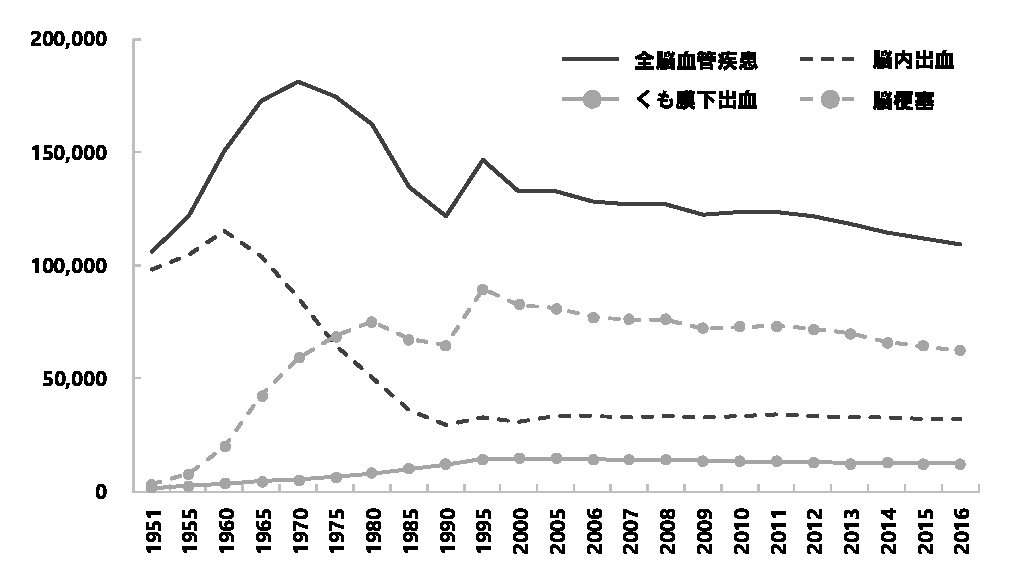
\includegraphics[width=0.95\linewidth]{./Chap1/fig/number_death.eps}
\caption{日本における脳卒中分類別死亡率の推移}
\label{fig:number_death}
\end{center}
\end{figure}

脳卒中のリハビリテーション(以下リハビリ)は,急性期,回復期,維持期の三つの区分に分けられている.
脳卒中発症直後の急性期からリハビリを行うことが勧められている\cite{脳卒中2009}.
脳卒中発症2週間後から5, 6ヶ月までの回復期において,
片側の上下肢が動かない片麻痺の患者は理学療法士から受けるリハビリを行うことで下肢の機能の再建を行う.
下肢機能の再建のための訓練により,Activities of Daily Livingの向上,Quality of Lifeの向上が見込める.
さらには維持期に長期的に運動機能を維持することで,社会復帰を図る.

%%%%%%%%%%%%%%%%%%%%%%%%%%%%%%%%%%%%%%%%%%%%%%%%%%%%%%%%%%%%%%%%%%%%%%%%%%%%%%%%%%%%%%%%%%%%%%%%%%%%%%%%%%%%%%%%%%%%%%%%%%%%%%%%%%%
\section{リハビリテーションへのロボットの介入}
\label{sec:robotics_chap1}
近年のロボット技術の向上により,リハビリの領域にロボットを介入することが期待されている.
ロボット介入の意義は
\begin{itemize}
	\item 多関節の同時コントロールが可能
	\item 正常軌道の運動が可能
	\item 負荷量の調節と負荷量の維持が可能
	\item 結果の提示,つまりフィードバックが可能
\end{itemize}
という4点である\cite{道免2015}.\\

すでに歩行運動については,歩行をアシストするロボットを用いることで歩行能力が改善された報告がある\cite{Fisher2011}\cite{Srivastava2016}\cite{有末2015}.

Fisherらは回復期の片麻痺患者に対し,理学療法士による従来のリハビリとアシストロボットを利用したトレッドミルでの歩行によるリハビリ(Robot Assisted Gait Trainig,以下RAGT)を比較した.
アシストロボット(Autoambulator)は患者を吊り下げるハーネスと,股関節・膝関節を補助する外骨格の駆動装置から成る.外観を図\ref{fig:autoambulator}に示す.
どちらの患者群でもリハビリの前後で,8 m歩行,3分歩行,Tinettiバランステストの全てにおいて優位にスコアが上昇した.
なお,理学療法士による従来のリハビリとRAGTによるリハビリとの間ではリハビリ後のスコアに差は無かった.

\begin{figure}[b]
	\begin{center}
		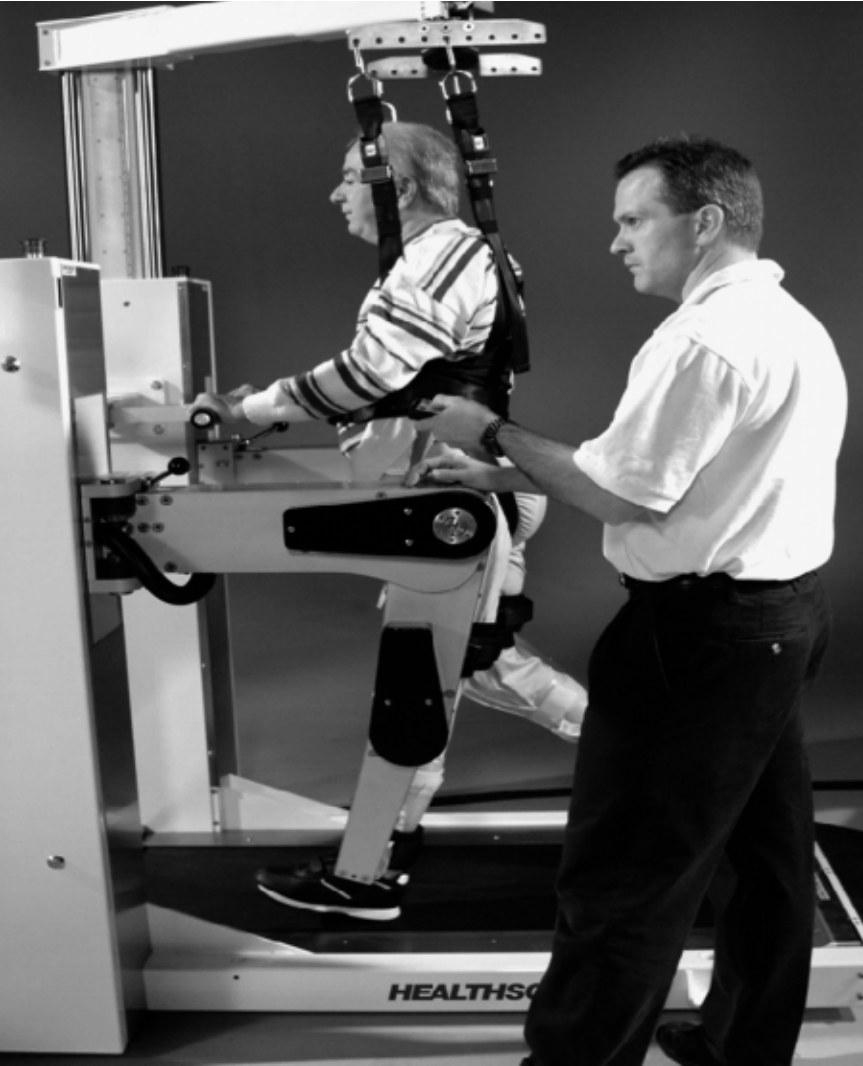
\includegraphics[width=4.5cm]{./Chap1/fig/Autoambulator.PNG}
		\caption{Autoambulatorによるリハビリの様子\cite{Fisher2011}}
		\label{fig:autoambulator}
	\end{center}
\end{figure}

Srivastavaらも理学療法士のリハビリとRAGTのリハビリを比較している.
麻痺側の足に外骨格(ALEX)を装着し,健常者の軌道から外れた時だけ支援する.
外観を図\ref{fig:ALEX}に示す.
Fisherらの結果と同様,どちらのリハビリでも患者の運動機能は改善したがスコアの上昇に差はなかった.
RAGTのリハビリの方が理学療法士の負担が減ると結論づけている.

\begin{figure}[b]
	\begin{center}
		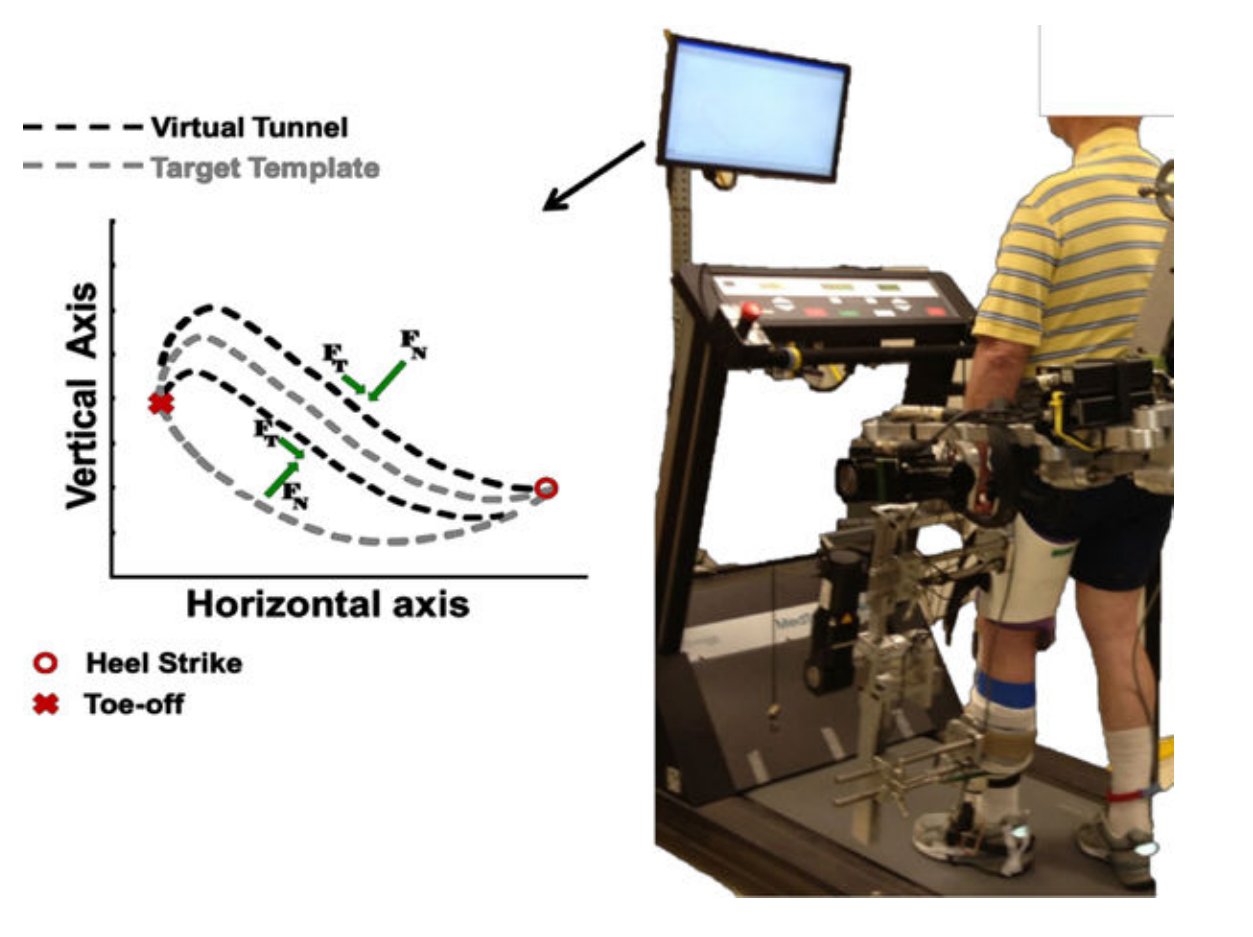
\includegraphics[width=8cm]{./Chap1/fig/ALEX.PNG}
		\caption{RAGTのリハビリの様子\cite{Srivastava2016}}
		\label{fig:ALEX}
	\end{center}
\end{figure}

有末らは回復期の片麻痺患者に対し,Honda歩行アシストを用いた歩行練習を検討した.
Honda歩行アシストは股関節の屈曲・伸展運動を大腿部のフラームを通じて補助する.
装着者の歩行周期に合わせて,股関節の屈曲・伸展のタイミングを補正する\cite{渡邊2016}.
訓練前の歩行速度が60 m/min未満の患者において,歩行速度や歩行の幅が増加した.\\

本研究では回復期のリハビリにおける片麻痺患者の起立動作に着目する.
運動機能が低下すると生活範囲が狭まる\cite{Guralnik1994}ため,日常生活の中で活動の起点となる起立動作の訓練が必要である.
入院中や退院後について理学療法士がいない中でも,廃用性症候群を防ぐために起立動作を行わなければならない.
よって,自立を促すための起立動作の支援への要求があり,片麻痺患者の起立動作を支援する機器の開発が重要である.
%次項にて起立動作の支援機器に関する従来研究について述べる.

\clearpage

%%%%%%%%%%%%%%%%%%%%%%%%%%%%%%%%%%%%%%%%%%%%%%%%%%%%%%%%%%%%%%%%%%%%%%%%%%%%%%%%%%%%%%%%%%%%%%%%%%%%%%%%%%%%%%%%%%%%%%%%%%%%%%%%%%%

\section{起立動作の支援機器に関する従来研究}
\label{sec:related_research_chap1}

起立動作の支援機器に関する従来研究について述べる.
%支援機器は大きく分けて2つに分類することができる.
多くの片麻痺患者は非麻痺側の足からの感覚入力が受け取れないため,姿勢制御が不安定になる\cite{Chou2003}.
そのため,健側の足に体重を乗せて立ち上がるので動作は左右で非対称なものとなり,健側の足に大きな負担がかかってしまう.
リハビリテーションにおいては麻痺側の足をいかに活用し,左右対称な動きにするかが重要である.

起立動作の支援機器の従来研究として,起立動作を外骨格などにより支援するもの\cite{Tsukahara2010}と座面が上昇することで支援するもの\cite{Shiraishi2016}がある.

TsukaharaらはロボットスーツHALを用いて完全片麻痺患者の起立動作を支援するシステムを開発した.
腰・膝・足関節の運動を支援するHALと,前方に倒れないようにするために腰をサポートするハーネスでシステムは構成されている.外観を図\ref{fig:HAL}に示す.
システムは脛が前傾し,足部の圧力中心がある閾値を超えるかどうか判断することで使用者の動作意図を読み取り,起立動作を支援する.
完全片麻痺患者1名に対して実験を行い,安定して立ち上がることができたと報告している.

\begin{figure}[b]
	\begin{center}
		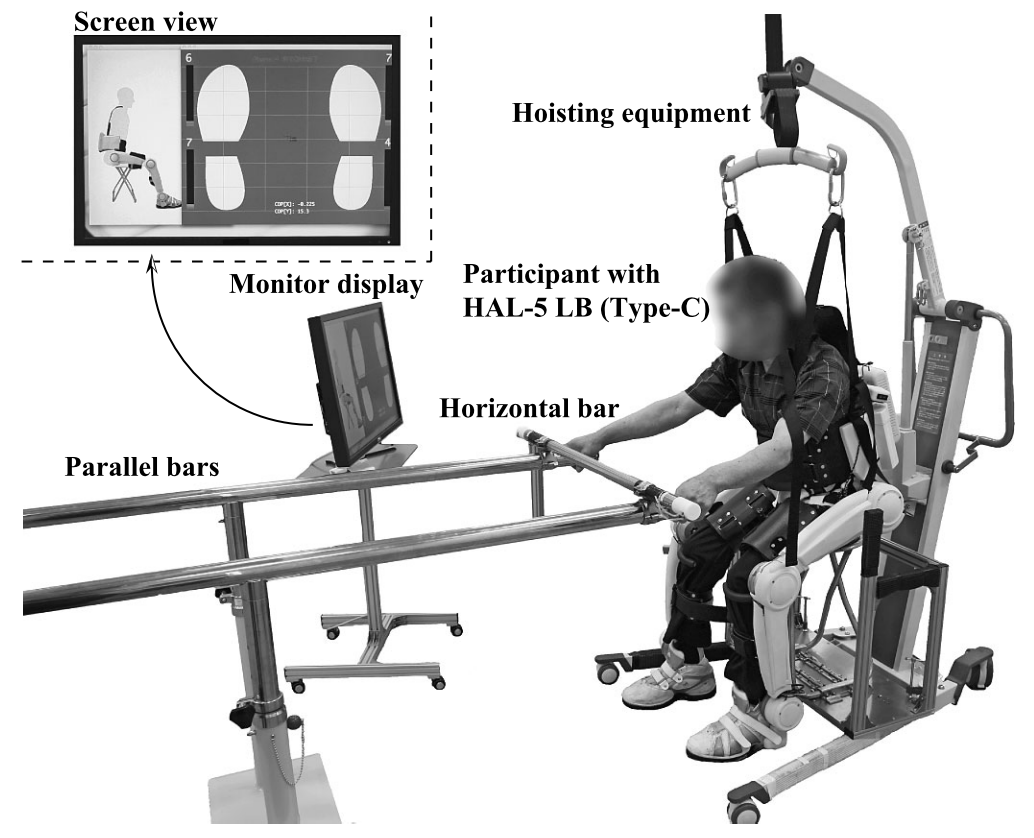
\includegraphics[width=10cm]{./Chap1/fig/HAL.PNG}
		\caption{HALを用いた支援の様子\cite{Tsukahara2010}}
		\label{fig:HAL}
	\end{center}
\end{figure}

Shiraishiらは座面が直線的に移動することで片麻痺患者の起立動作を支援するシステムを開発した.
床反力から使用者の動作意図を読み取り,座面が臀部を直線的に押し上げることで起立動作を支援する.外観を図\ref{fig:Handrail}に示す.
2名の片麻痺患者と1名の四肢麻痺患者に対して実験を行い,麻痺側と非麻痺側の足の使用率の差が減少したと報告している.

\begin{figure}[b]
	\begin{center}
		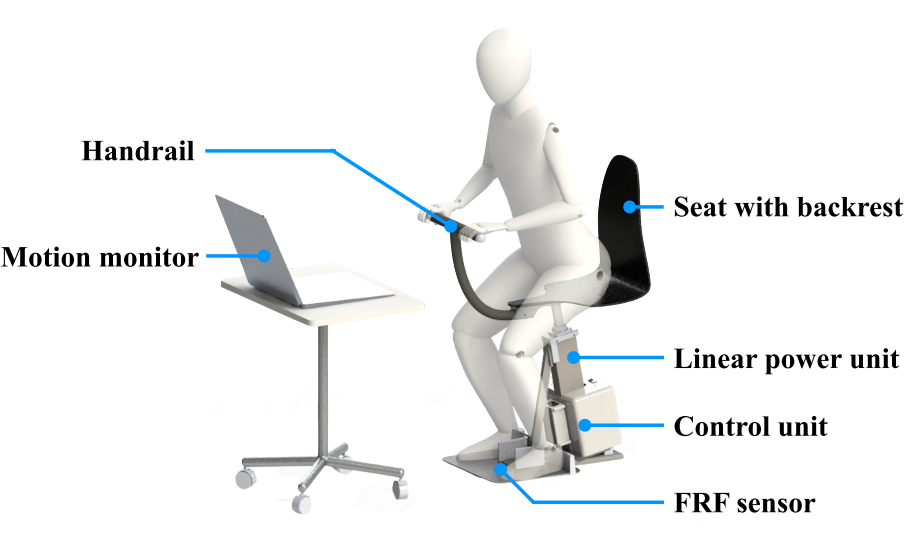
\includegraphics[width=10cm]{./Chap1/fig/Handrail.PNG}
		\caption{支援の様子\cite{Shiraishi2016}}
		\label{fig:Handrail}
	\end{center}
\end{figure}


これらの従来研究は関節に力を補助するような筋力増強が主である.
運動を最初から最後まで支援することなり,支援のしすぎとなる可能性がある.
しかし,運動を支援する際には,運動のメカニズムを理解したうえで支援することが重要である.



\clearpage
%%%%%%%%%%%%%%%%%%%%%%%%%%%%%%%%%%%%%%%%%%%%%%%%%%%%%%%%%%%%%%%%%%%%%%%%%%%%%%%%%%%%%%%%%%%%%%%%%%%%%%%%%%%%%%%%%%%%%%%%%%%%%%%%%%%
\section{研究の目的}
\label{sec:objective_chap1}

\ref{sec:background_chap1}節で,脳卒中により片麻痺となった患者のリハビリの重要性について述べた.
\ref{sec:robotics_chap1}節で,歩行動作のリハビリに投入されるロボットについて,\ref{sec:related_research_chap1}節で起立動作の支援機器について述べた.
しかし,従来の支援機器ではヒトの運動のメカニズムを理解した上で動作を支援していないことが明らかになった.\\

本研究ではヒトの運動のメカニズムを理解し,片麻痺患者のリハビリを日常的に支援する機器を開発する.
本研究の対象者は回復期の片麻痺患者であり,入院中に日常的に使用することでリハビリを行うことを目指す.
まず,片麻痺患者が理学療法士によるリハビリを受けてどのように起立動作が変化するかを調査する.
起立動作の変化をヒトの運動のメカニズムに沿って捉えることで,リハビリの効果を検証する.
次に,片麻痺患者の起立動作のリハビリにおける理学療法士の技能を解析する.
理学療法士は片麻痺患者の起立動作の最初から最後まで力を入れているわけではなく,特定のタイミングで起立動作を支援している.
特定のタイミングで支援する技能を解析することで,起立動作の支援機器に応用する.
そして,起立動作の支援機器を開発し,機器の有効性を検証する.

以上より,本研究の目的を以下のように3つ設定する.
%\begin{center}
%\doublebox{
%	\begin{tabular}{c}
		\begin{enumerate}
			\item 理学療法士の介入による片麻痺患者への影響を調査
			\item 理学療法士の技能を解析
			\item 理学療法士の技能を活用した,起立動作の支援機器の開発
		\end{enumerate}
%	\end{tabular}
%}
%\end{center}





\clearpage


%%%%%%%%%%%%%%%%%%%%%%%%%%%%%%%%%%%%%%%%%%%%%%%%%%%%%%%%%%%%%%%%%%%%%%%%%%%%%%%%%%%%%%%%%%%%%%%%%%%%%%%%%%%%%%%%%%%%%%%%%%%%%%%%%%%
\section{本論文の構成}

本論文は全6章から構成されている.本論文の構成を図\ref{fig:thesis_flow}に示す.

第1章では,本研究の背景と従来研究,目的について述べた.

第2章では,問題設定を明らかにし,本研究におけるアプローチについて述べる.

第3章では,理学療法士のリハビリテーションによる片麻痺患者への影響について述べる.

第4章では,理学療法士のリハビリテーションの技能について述べる.

第5章では,起立動作の支援機器への応用と有効性を検証するために行った実験について述べる.

第6章では,本研究の結論と今後の展望について述べる.

%\clearpage


\begin{figure}[b]
\begin{center}
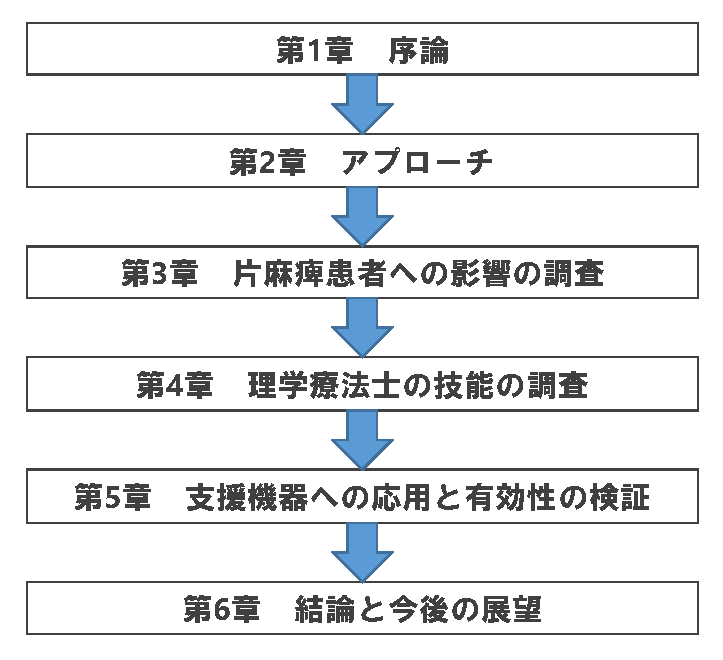
\includegraphics[width=8cm]{./Chap1/fig/thesis_flow.eps}
\caption{本論文の構成}
\label{fig:thesis_flow}
\end{center}
\end{figure}

\clearpage



%%%%%%%%%%%%%%%%%%%%%%%%%%%%%%%%%%%%%%%%%%%%%%%%%%%%%%%%%%%%%%%%%%%%%%%%%%%%%%%%%%%%%%%%%%%%%%%%%%%%%%%%%%%%%%%%%%%%%%%%%%%%%%%%%%%
%%% Local Variables:
%%% mode: katex
%%% TeX-master: "../thesis"
%%% End:
